\documentclass[11pt]{article}
\usepackage{hyperref}
\usepackage[english]{babel}
\usepackage{blindtext}
\usepackage{url}
\usepackage{graphicx}
\usepackage{multicol}
\usepackage[center]{titlesec}
\usepackage{geometry}
\usepackage{lettrine} % The lettrine is the first enlarged letter at the beginning of the text

%\usepackage{mathtools}

\usepackage[sort, numbers]{natbib}


%
%\setlength{\columnseprule}{0.4pt}
%\setlength{\footskip}{20pt}
\usepackage{fancyhdr}
\fancyhf{}
\fancyhead[C]{ $\bullet$ Weather data $\bullet$ }
\fancyfoot[C]{  $\bullet$ Uganda \bullet$  }
\renewcommand\headrulewidth{1pt}
\renewcommand\footrulewidth{1pt}
\pagestyle{fancy}

%

\setlength{\columnsep}{1.5cm}
%\setlength{\columnseprule}{0.4pt}

%\MakeOuterQuote{"}



\graphicspath{ {/home/joebrew/Documents/weather/uganda/uganda_weather_first_pass} }

%the next two lines adjust the third, centered section of the exec sum
\def\changemargin#1#2{\list{}{\rightmargin#2\leftmargin#1}\item[]}
\let\endchangemargin=\endlist 

\usepackage{Sweave}
\begin{document}
\Sconcordance{concordance:uganda_weather_first_pass.tex:uganda_weather_first_pass.Rnw:%
1 42 1 1 0 8 1 1 21 1 3 83 1 1 75 1 2 1 1 1 75 1 2 44 1}


\title{\textbf{Ugandan Weather: First Pass}}
\author{Joe Brew}

\maketitle

\begin{center}
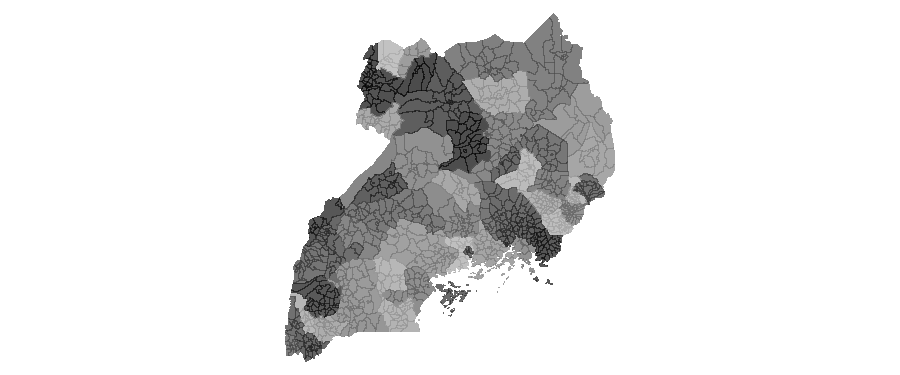
\includegraphics{uganda_weather_first_pass-001}
\end{center}

\begin{center}

\includegraphics[width=2cm]{logo}
\end{center}


\emph{\noindent The following is a brief overview of a first attempt to systematically collect Ugandan weather-related data.  I outline the code I used to capture the data, describe the data's quality, summarize the method's flaws, and propose some options for improving this process. }
\tableofcontents

\vspace{10mm}



\newgeometry{margin=2.2cm}
%\fancyhfoffset[E,O]{0pt}


%------------------------------------------
\section*{Webscraping Ugandan weather data}
\addcontentsline{toc}{section}{Webscraping Ugandan weather data}
%------------------------------------------
\hrulefill

\begin{multicols}{2} 
\setkeys{Gin}{width=0.45\textwidth}

%------------------------------------------
\subsection*{Method}
\addcontentsline{toc}{subsection}{Method}
%------------------------------------------

\lettrine[nindent=0em,lines=3]{I}{} wrote some \href{https://github.com/joebrew/weather/tree/master/uganda}{code} in R to scrape historical Ugandan weather data directly from the \href{http://wunderground.com}{Weather Undeground website}. The scrape\_data() function takes a location, start date, end date and airport boolean\footnote{Weather Underground's URLs are oddly different for airport and non-airport locations} and returns a format-standardized dataframe (R object) which can easily be written to a transportable file (.csv, .txt, etc.): 
\begin{verbatim} 
scrape_data(station = "ICENTRAL28", 
            start_date = Sys.Date() 
                          - 365,
            end_date = Sys.Date(),
            airport = TRUE)) 
\end{verbatim} 

The data returned consist of daily observations of precipitation, temperature, humidity, cloud cover, and dew point.  \\

I also cobbled together \href{https://github.com/joebrew/weather/blob/master/uganda/visualization_functions.R}{a few plotting functions} to visualize variation in these indicators over time and space (see charts after report).

%------------------------------------------
\subsection*{Results}
\addcontentsline{toc}{subsection}{Results}
%------------------------------------------
Results are mediocre.  Of the 15 total Ugandan locations available in Wunderground's search options, only 4 appear to have functioning weather stations, of which 3 are in the same area (Kampala). \\

Data from Kampala appear to be of relatively high (usable) quality, especially if we supplement Kampala-area data to supplement on days in which data are missing.  Data from Soroti (a medium-sized town about 200km to the Northwest of Kampala) are also decent.  In both locations, precipitation data appear unreliable (far too low).

%------------------------------------------
\subsection*{Advantages and shortcomings}
\addcontentsline{toc}{subsection}{Advantages and shortcomings}
%------------------------------------------
\noindent \textbf{Advantages:} Multiple weather-related indicators from two areas of Uganda are readily-available and easily accessed.  This method of directly scraping is simple enough that it could be implemented easily and scheduled to update regularly.  This did not require use of Wunderground's API (which is relatively restrictive).  \\

\noindent \textbf{Shortcomings:} This method assumes the user knows the name and type of weather stations of interest. Given that it's not API-based, it is subject to formatting changes at any time.  Only two geographic locations in Uganda have valuable data.  Data quality/precision has not been assessed.

%------------------------------------------
\subsection*{Moving forward}
\addcontentsline{toc}{subsection}{Moving forward}
%------------------------------------------
This first pass demonstrated that historical location-specific weather data are relatively easy to capture.  Moving forward, we'll need to \begin{itemize}
\item Explore other weather data sources for more granularity within Uganda (since Wunderground is limited in this).
\item Develop future code in a way that doesn't require \emph{a priori} knowledge regarding weather station nomenclature, etc. (ie, functions to take a location and return nearest weather, with some quantification of uncertainty).
\item Consider using an API and integrate weather data grabs directly into the app (necessary if we want to make weather a feature of many projects, unnecessary if we choose to incorporate weather on a project-specific basis).
\item Test whether weather data is even predictive! And if it is, use caution in how we model with it - in the case of solar units, raininess might be correlated with increased risk of non-payment (less revenue generation), but severe spikes in raininess might correlate with power outages (which could be good for business).  
\end{itemize}


\newgeometry{margin=0.5cm}
\end{multicols}
\setkeys{Gin}{width=1\textwidth}

%------------------------------------------
\section*{Visuals}
\addcontentsline{toc}{section}{Visuals}
%------------------------------------------
\hrulefill

\begin{center}
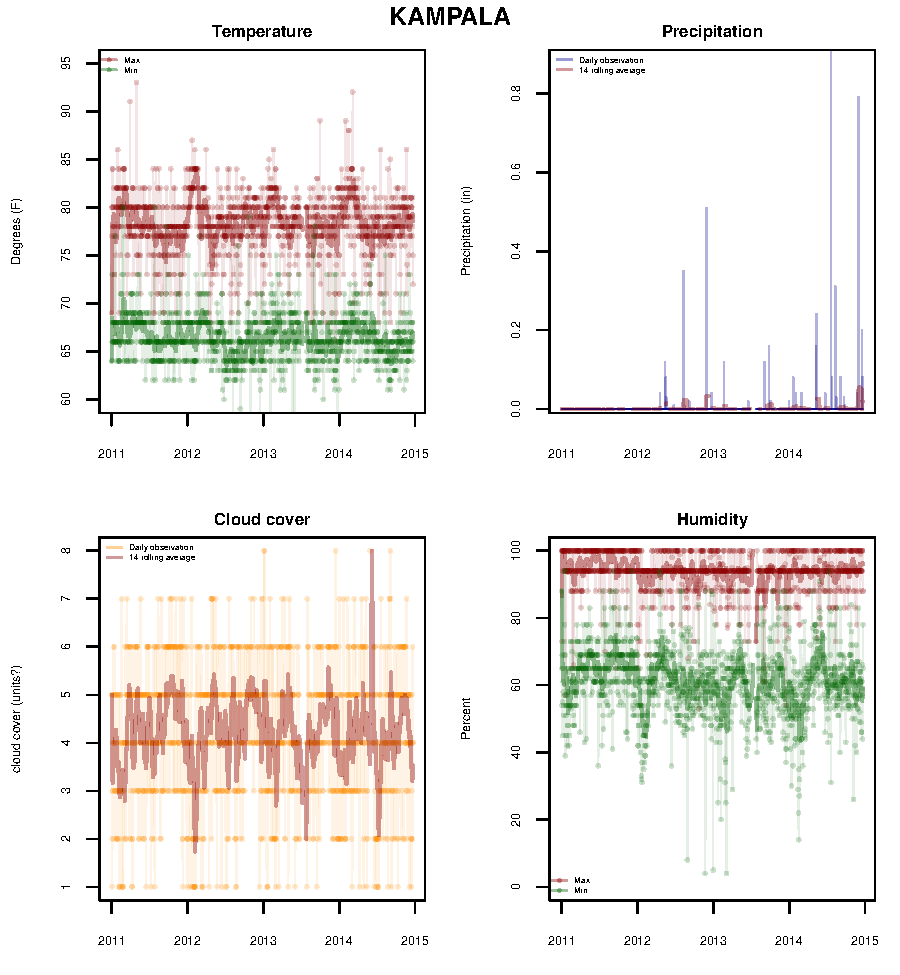
\includegraphics{uganda_weather_first_pass-002}


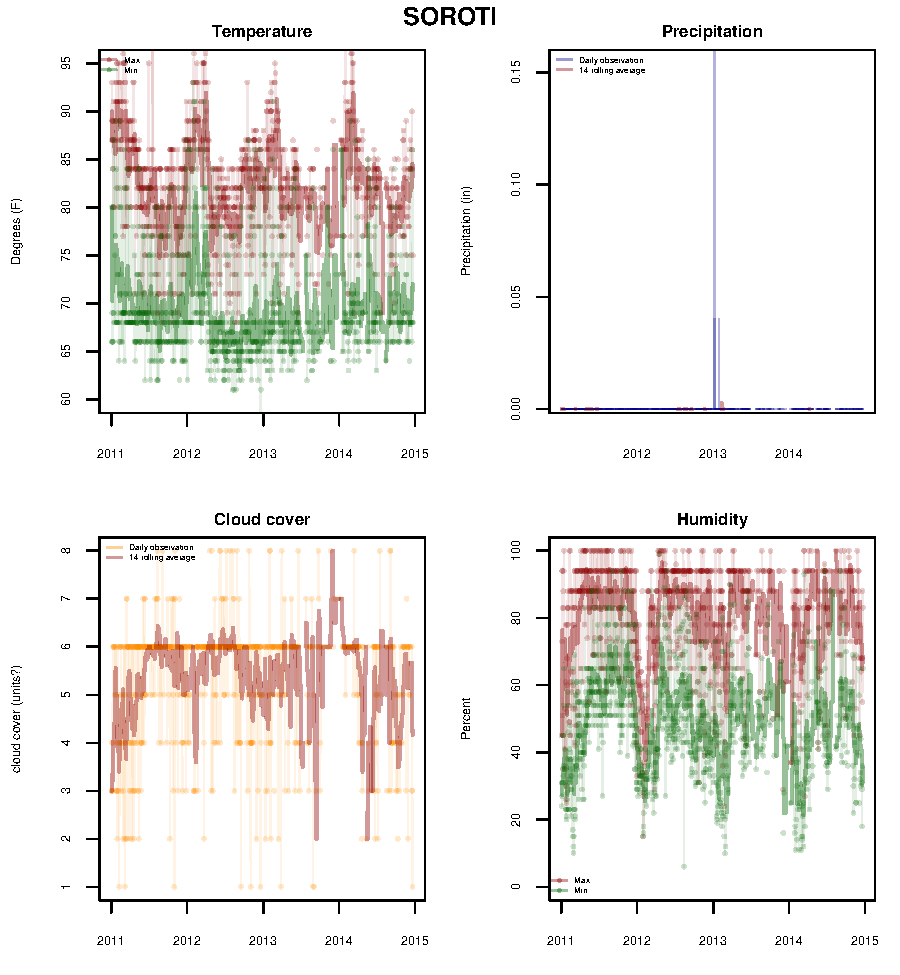
\includegraphics{uganda_weather_first_pass-003}
\end{center}

\newpage
%------------------------------------------
\section*{Details}
\addcontentsline{toc}{section}{Details}
%------------------------------------------
\hrulefill

Full code at \href{https://github.com/joebrew/weather/tree/master/uganda}{https://github.com/joebrew/weather/tree/master/uganda}: 
\begin{itemize}
\item \href{https://github.com/joebrew/weather/blob/master/uganda/scrape_data.R}{Function to scrape data}
\item \href{https://github.com/joebrew/weather/blob/master/uganda/uganda_weather.csv}{4 years of Ugandan weather data}
\item \href{https://github.com/joebrew/weather/blob/master/uganda/visualization_functions.R}{Some clunky weather plotting functions}
\item \href{https://github.com/joebrew/weather/blob/master/uganda/visualization_interactive.R}{Slightly less clunky, interactive weather-plotting functions}
\item \href{https://github.com/joebrew/weather/blob/master/uganda/gadm.R}{Code to grab shapefiles from anywhere in the world}
\item \href{https://github.com/joebrew/weather/tree/master/uganda_weather_first_pass}{Code used for this report} \\
\end{itemize}

Weather undeground resources: \begin{itemize}
\item \href{www.wunderground.com}{Weather underground} 
\item \href{http://www.wunderground.com/weather/api/}{Weather underground's API page} \\
\end{itemize}

Resources I haven't looked into in detail yet (but will): \begin{itemize}
\item \href{http://openweathermap.org/history}{Openweathermap: Free historical weather API}
\item \href{http://www.worldweatheronline.com/api/local-city-town-weather-api.aspx}{Worldweatheronline: looks sketchier}
\item \href{https://developer.yahoo.com/weather/#get-started}{Yahoo's weather API}
\item \href{http://www.programmableweb.com/news/26-weather-apis-12-support-json/2012/01/11}{Page with lots of weather API resources I haven't looked into yet} \\
\end{itemize}

This report was generated on \today.  The author used R version 3.1.2 (2014-10-31) (Pumpkin Helmet) on a linux-gnu OS.  \\

The analysis in this report was written in the R programming language, and the report production was programmed in \LaTeX{} using Sweave.\\


%----------------------------------------------------------------------------------------
%  REFERENCE LIST
%----------------------------------------------------------------------------------------
% \newpage
% \bibliographystyle{unsrtnat}
% \bibliography{bibliography}


\end{document}
